\chapwithtoc{Attachments}

\section*{CD contents}\label{cd-contents}

The compact disk attached to this thesis contains the following:

\begin{itemize}
\item \verb+thesis.pdf+, the PDF version of this thesis;
\item \verb+TransportEditor/+, the \TEver{} release (Git Tag \TEtag{}) of the TransportEditor software, also obtainable at:\\
\url{https://github.com/oskopek/TransportEditor/releases}. Contains:
\begin{itemize}
\item \verb+datasets/+, the datasets used at IPC;
\item \verb+docs/+, the user, developer, and JavaDoc documentation and a specification document for TransportEditor;
\item \verb+sources/+, sources of TransportEditor along with source of planners, benchmarks and the report generator; and
\item \verb+tools/+, the benchmarker execution scripts and configuration files, along with other tools used. The folder \verb+tools/benchmarks/results+ contains the benchmark results
from Sections~\ref{sequential-results} and~\ref{temporal-results}.
\end{itemize}
\end{itemize}

\subsection*{TransportEditor User Manual}\label{transporteditor-user-manual}

A user manual explaining use-cases, the user interface, saving and loading files,
and other actions is also available on the attached CD, in the folder:\\
\verb+TransportEditor/docs/manuals/+.

\subsection*{TransportEditor Developer Manual}\label{transporteditor-developer-manual}

A developer manual explaining the architecture, technical choices, and program flow
is also available on the attached CD, in the folder:\\
\verb+TransportEditor/docs/manuals/+.

\subsection*{TransportEditor Developer JavaDoc}\label{transporteditor-developer-javadoc}

Generated API documentation using JavaDoc is also available on the attached CD, in the folder:\\
\verb+TransportEditor/docs/javadoc+.

\newpage

\section*{TransportEditor --- A Transportation Planning System}

To enable effective transportation planning,
we have developed \textit{TransportEditor}, a system for creating and visualizing transportation problems and plans.
Specifically, TransportEditor aims to be a problem editor and plan visualizer for the Transport domain (and its variants). It is an intuitive and cross-platform graphical desktop application (Figure~\ref{fig:transporteditor-screenshot})
written in Java.

It allows the users to create a planning session, where they
select a Transport domain variant, load a problem instance from PDDL (Section~\ref{pddl}) or create a new one from scratch.
The road network of the problem is automatically laid out and visualized for the users as a graph with locations as nodes and roads as edges.
Users can then tweak the layout, make changes to vehicle and package properties
and export the problem or domain back into PDDL.

They can also select an external planner
referencing its executable file, or select one of the built-in planners and try to solve
the loaded problem using the selected planner. Internal and external plan validators, like VAL \citep{Howey2003}, can also be selected to verify that the plans are correct.
Once plans are loaded and verified, it will let the users see a list of actions
in the plan, or plot a Gantt chart, which is useful for observing concurrent actions in temporal domain variants (Figure~\ref{fig:tempo-sat-6-gantt}).

The best feature of TransportEditor is the option of tracing plans. We can select
any action, specify an exact time point or just step through the actions in order and
the road network on the left will display the current state of the problem, as if
all actions before the current point were applied to the start state.
It is possible to do all of this, and more, without ever leaving the TransportEditor user interface.

TransportEditor will help researchers working on this domain fine-tune their planners; they can visualize the various corner cases their planner fails to handle, step through the generated plan and find the points where their approach fails.
A secondary motivation is to be able to test approaches for creating plans for the domain.
For screenshots of typical TransportEditor usage, see the attached \nameref{transport-editor-screenshots}.

\begin{figure}[t]
\begin{center}
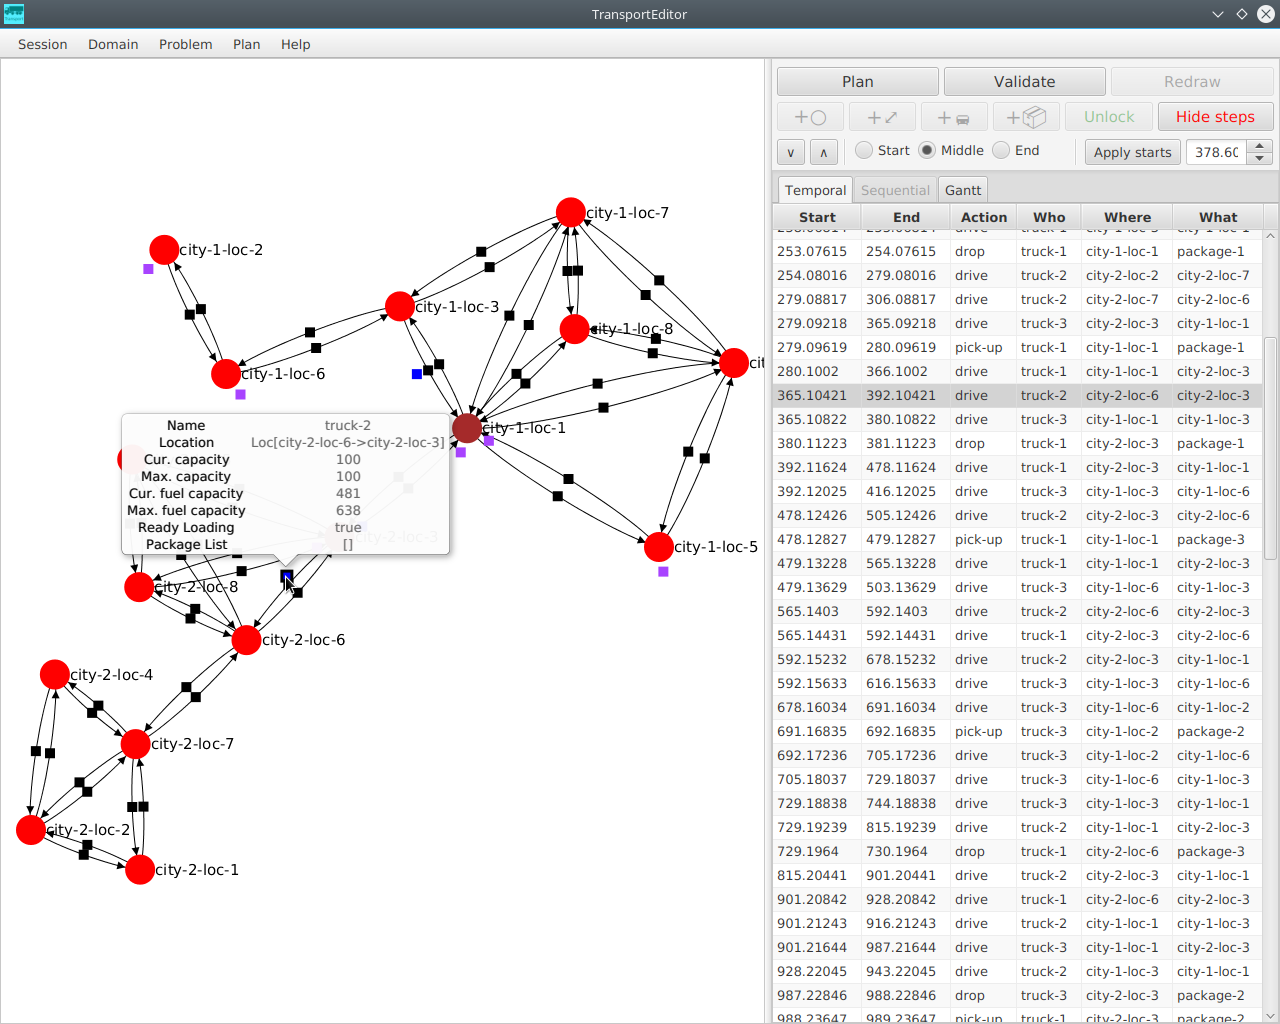
\includegraphics[width=0.9\textwidth]{../img/transporteditor_temporal}
\end{center}
\caption*%[Screenshot of a user tracing actions of a plan for a small temporal problem in TransportEditor.]
{Screenshot of a user tracing actions of a plan for a small temporal problem in TransportEditor. The bubble in the middle shows details
of a truck currently driving along a road between \texttt{city-2-loc-6} and \texttt{city-2-loc-3}. The \texttt{city-1-loc-1} location is plotted in a darker shade of red, which signifies that a petrol station is present at the location.}
\label{fig:transporteditor-screenshot}
\end{figure}

The basic user workflow of TransportEditor consists of the following steps:
\begin{itemize}
\item Selecting which formulation of the Transport domain they want to work with or create their own variant;
\item Loading the PDDL or creating their own problem of the given domain. TransportEditor then visualizes the given graph as good as it can;
\item Iterating among the following options:
\begin{itemize}
\item Loading a planner executable and letting TransportEditor run the planner on the loaded problem instance for a given time (the user can cancel anytime),
then loading the resulting plan;
\item Possibly loading a pregenerated plan;
\item Stepping through the individual plan actions and letting TransportEditor visualize them.
The user can step forward and backward in the plan and inspect each action result in great detail;
\item Editing the graph: adding/removing/editing the location or properties of vehicles, packages, roads, locations and possibly petrol stations;
\item Saving the currently generated plan;
\item Saving the problem or domain (exporting to a PDDL file).
\end{itemize}
\item Exit the application or go back to the first step.
\end{itemize}

TransportEditor is a part of this thesis and the reader can find it on the attachment CD (see the attached \nameref{cd-contents} for more information). Both the \nameref{transporteditor-user-manual},
the \nameref{transporteditor-developer-manual}, and the \nameref{transporteditor-developer-javadoc} are attached to this thesis in a digital format, offering guidance when
using the program and providing an in-depth description.

\newpage

\section*{TransportEditor screenshots}\label{transport-editor-screenshots}

Additional screenshots displaying typical TransportEditor usage.
\medskip

\begin{center}
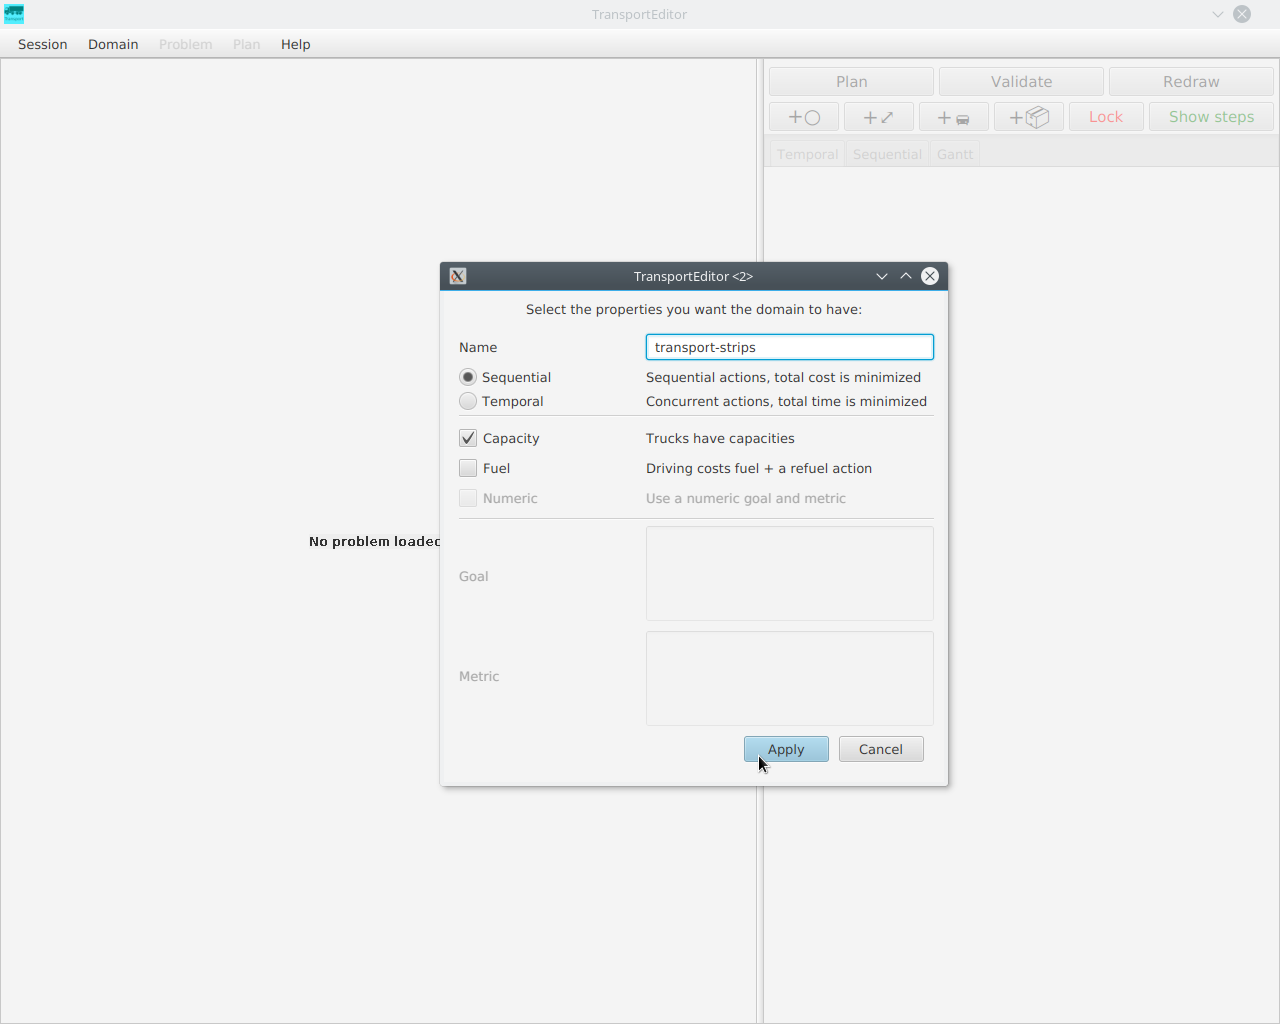
\includegraphics[width=0.91\textwidth]{../img/transporteditor_dom-creat}
Selecting a domain variant.
\end{center}
\medskip

\begin{center}
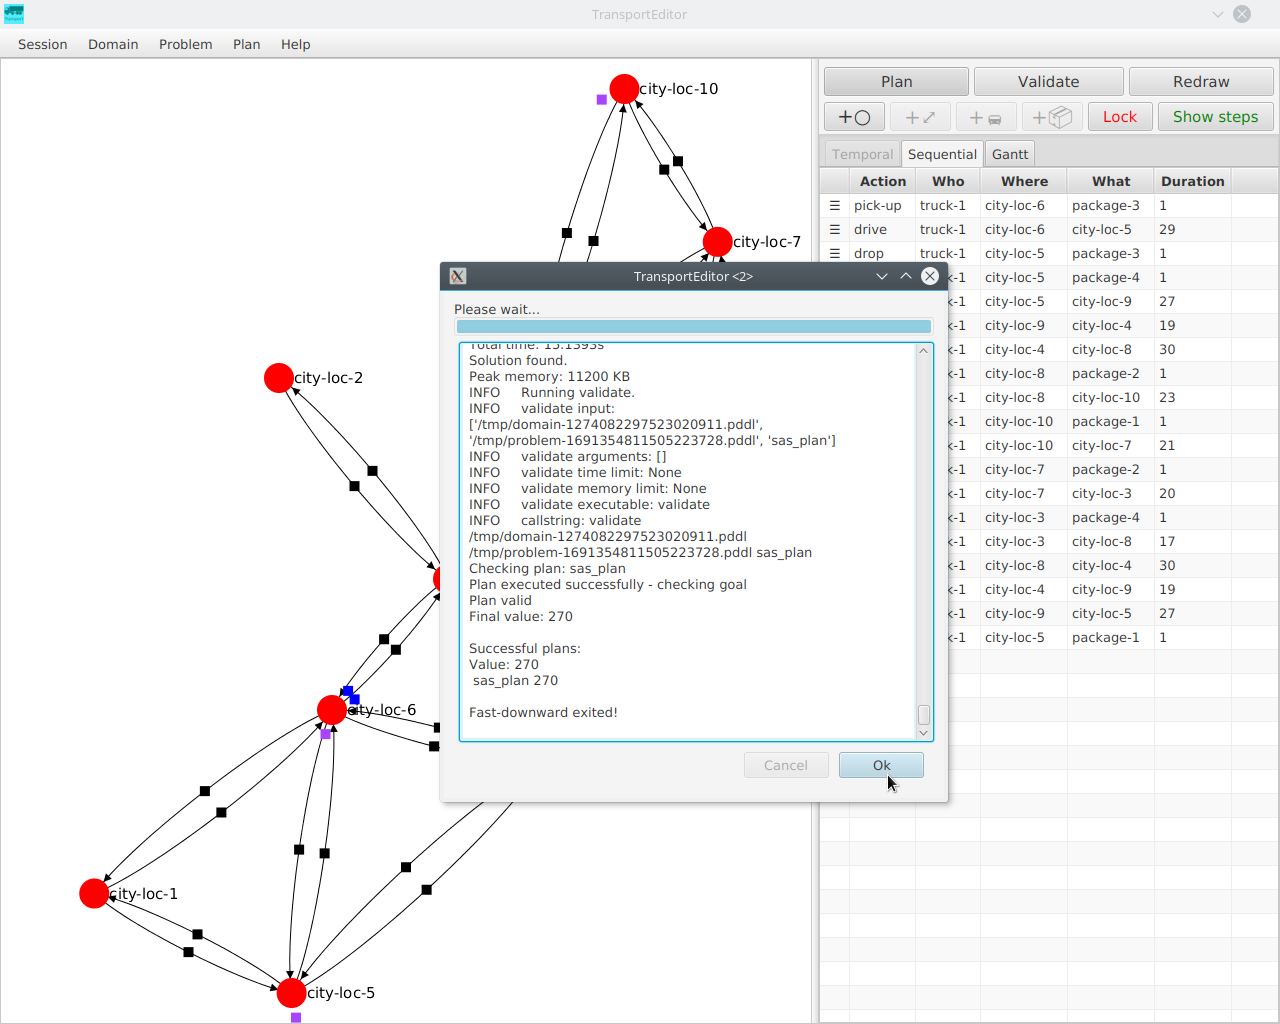
\includegraphics[width=0.91\textwidth]{../img/transporteditor_planning}
Running an external planner on a sequential problem.
\end{center}
\medskip

\begin{center}
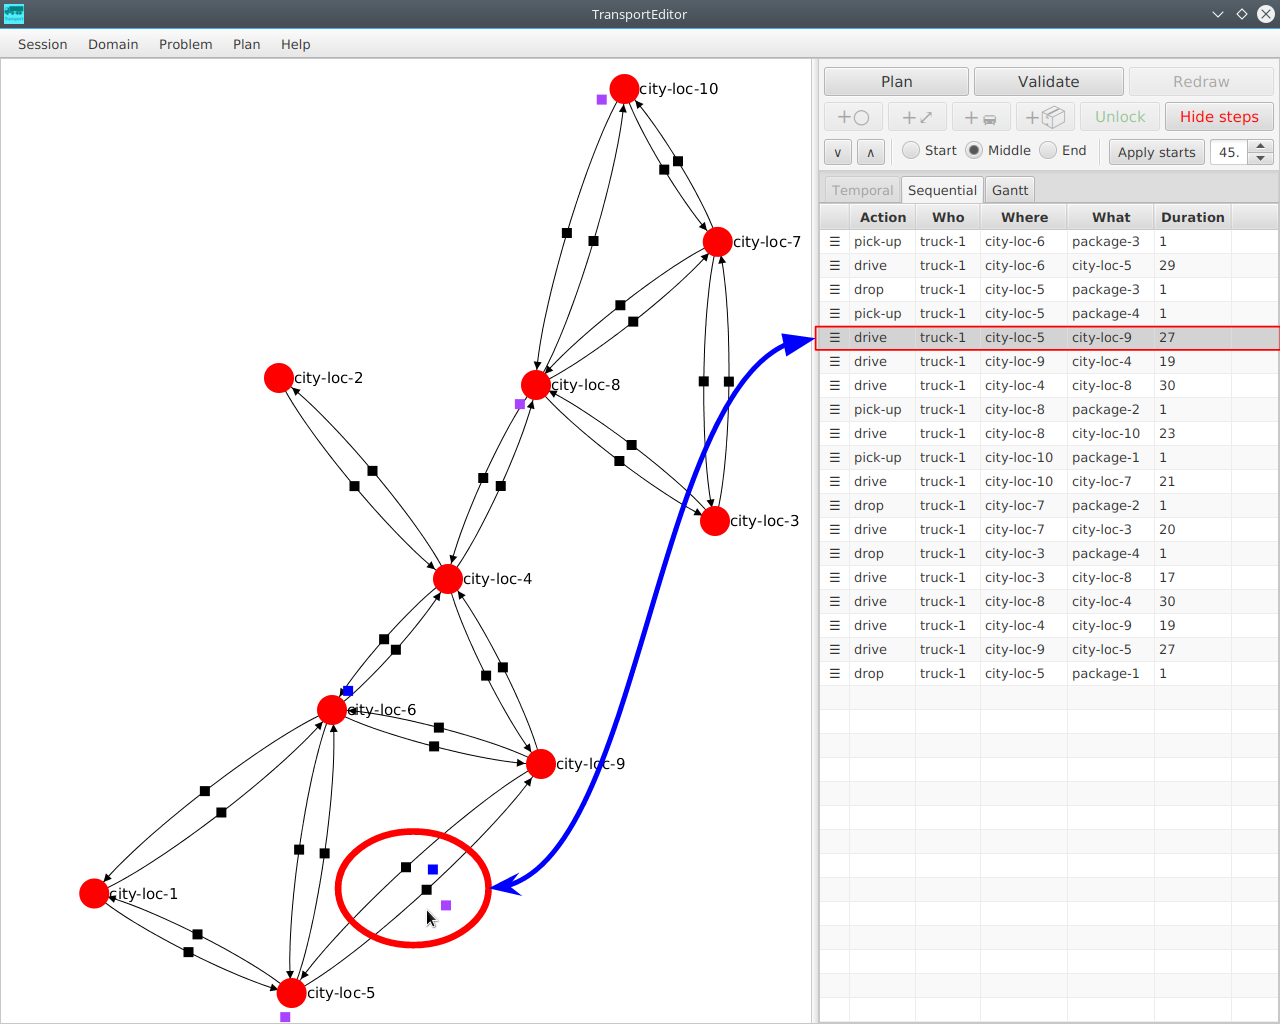
\includegraphics[width=0.94\textwidth]{../img/transporteditor_planstates}
Tracing a sequential plan. Highlighted is the corresponding \verb+drive+ action and the visualization of the vehicle (blue square) and the package it carries (purple square) on the road graph.
\end{center}
\medskip

\begin{center}
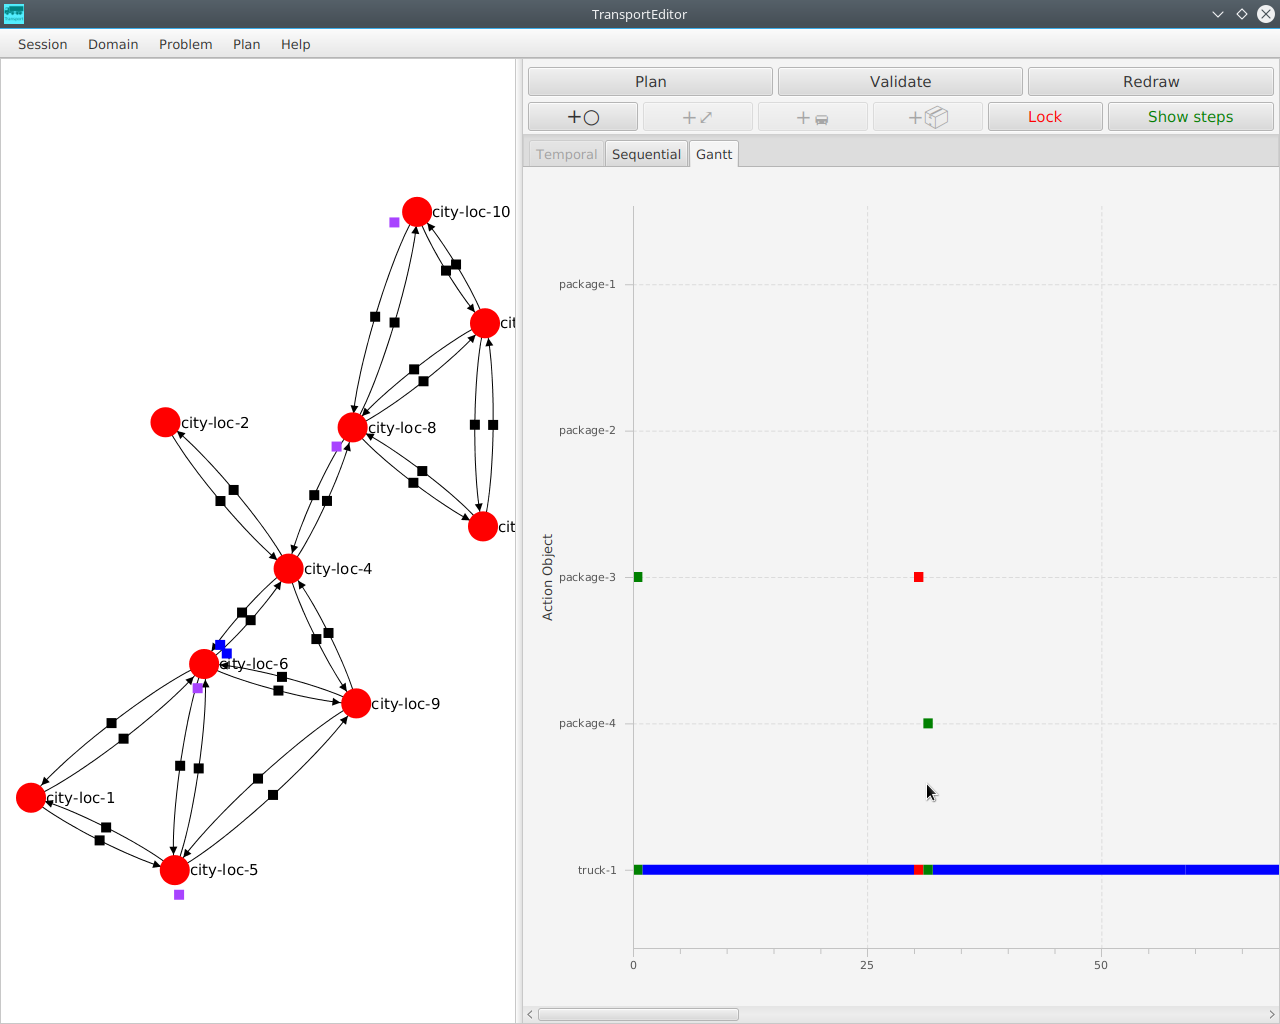
\includegraphics[width=0.94\textwidth]{../img/transporteditor_gantt}
Visualizing the plan as a Gantt chart.
\end{center}

\newpage

\section*{Accompanying software toolkit architecture}\label{transport-project}

To run our experiments efficiently, we have implemented a software project,
confusingly called TransportEditor, of which the editor described in
the previous section is only a part.
The ``scaffolding'' for running experiments, generating reports, and the planner implementations that we will describe in the next two chapters are all part
of the project as well.

The project is split into several modules, listed in approximate dependency order:
\begin{itemize}
\item \texttt{transport-thirdparty}, a set of 3$^\textrm{rd}$ party libraries
that have not been published in a dependency management repository like Maven~Central,\footnote{\url{http://central.sonatype.org/}}
making their compile-time download and linking impossible;
\item \texttt{transport-core}, a module that contains code modeling the Transport
domain and persisting it to disk;
\item \texttt{transport-planners}, containing sequential and temporal planners, both \textit{internal} (implemented as a part of this project) and \textit{external}
(only calling an executable of a different project);
\item \texttt{transport-benchmark}, a set of tools for running repeatable
experiments on Transport datasets, possibly in parallel;
\item \texttt{transport-report}, a collection of table generators and graph plotters,
operating on the results of benchmarks; and
\item \texttt{transport-editor}, the module containing the graphical user interface
of the planning system TransportEditor. This module is only dependent
on \texttt{transport-planners} and all its dependencies.
\end{itemize}
Independent on the other modules is \texttt{transport-docs},
the module containing this thesis,
along with our other textual works relating to researching the Transport domain.

Information about the model in \texttt{transport-core} and the \texttt{transport-editor} is available in the \nameref{transporteditor-user-manual} and the \nameref{transporteditor-developer-manual}.

All the modules are written in Java and attached to this thesis (see \nameref{cd-contents} for details). Also included are a few shell scripts, usually for quick
data conversion. The only important scripts reside in the \texttt{tools} folder;
the \texttt{benchmark.sh} script, used for running experimental benchmarks,
and \texttt{generate-reports.sh}, used for generating SVG and PDF plots or \LaTeX tables of the scores and runtimes from benchmark results.

The benchmarker takes as input a JSON \citep{Bray2014} configuration file (Figure~\ref{code:benchmark-config-bnf}),
runs the specified benchmarks and returns a \texttt{results.json} output file in a different JSON format (Figure~\ref{code:benchmark-results-bnf}).
In both of the figures are BNF grammars. We write zero-or-more repeated statements using ( and )*. Also, [ and ] are used for JSON lists, they do not mean an optional statement --- we use ( and ) (without the star) for that.
Under \texttt{<character>}, we assume any valid UTF-8 character,
\texttt{<double>} means any non-negative IEEE compatible double precision floating-point number,
and \texttt{<long>} is any non-negative whole number smaller than or equal to $2^{63}-1$.
Additionally, all file paths may use the \verb+${transport.root}+ variable, designating the
root directory of the project.

Apart from the results file, a plain text log containing information about the planner
runs is also produced. Both of these files are placed in the directory \texttt{results/config\_file\_name/YYYYmmdd-HHMMSS/}, under the directory where \texttt{benchmark.sh} is placed.
We can then use the \texttt{generate-reports.sh} script on the results file,
which will create a \texttt{reports} directory next to the results file,
containing all the generated report files.

\begin{figure}[tbp]
\centering
\begin{code}
<config> ::= { "domain" : "<filepath>",
               "problems" : { "<problem_name>" : <problem_config>
                          ( , "<problem_name>" : <problem_config> )* },
               "scoreFunctionType"  : "<score_function>",
               "planners": { "<planner_name>" : "<planner_config>"
                        ( , "<planner_name>" : "<planner_config>" )* },
               "threadCount": <integer>,
               "timeout": <integer> }
<filepath> ::= <string>
<problem_name> ::= <string>
<problem_config> ::= { "filePath" : "<filepath>",
                       "bestScore" : <score> }
<score> ::= null | <float>
<score_function> ::= TOTAL_TIME | ACTION_COUNT
<planner_name> ::= <string>
<planner_config> ::= { "className" : "<class>",
                       "params" : "<executable_templ>" }
<class> ::= <string>
<executable_templ> ::= <string>
<string> ::= ( <character> )*
\end{code}
\caption*%[Grammar of the input configuration JSON file in BNF.]
{Grammar of the input configuration JSON file in BNF. The token \texttt{<class>}
is expected to be a valid Java class name (including the package) and present on the classpath.
The \texttt{<executable\_templ>} token is expected to be a valid executable planner with supplied parameters
and \{0\} used to represent the domain file path, \{1\} the problem file path, and \{2\} the output plan file path.}
\label{code:benchmark-config-bnf}
\end{figure}

\begin{figure}[tbp]
\centering
\begin{code}
<results> ::= { "runs" : [ ( <run> ) ( , <run> )* ] }
<run> ::= { "actions" : [ ( <action> ) ( , <action> )* ],
            "temporalPlanActions" : [ ( <tpa> ) ( , <tpa> )* ],
            "domain" : "<string>",
            "planner" : "<string>",
            "problem" : "<string>",
            "results" : <run_results> }
<action> ::= "<string>"
<tpa> ::= "<string>"
<run_results> ::= { "score" : <score>,
                    "bestScore" : <score>,
                    "exitStatus" : "<exit_status>",
                    "startTimeMs" : <timestamp>,
                    "endTimeMs" : <timestamp>,
                    "durationMs" : <timestamp>,
                    "quality" : <double> }
<exit_status> ::= UNSOVLED | INVALID | VALID | NOTVALIDATED | SUBOPT
<timestamp> ::= <long>
\end{code}
\caption*%[Grammar of the input configuration JSON file in BNF.]
{Grammar of the input configuration JSON file in BNF.
The tokens \texttt{<action>} and \texttt{<tpa>} were defined in Section~\ref{pddl}. Note
that this grammar is only valid if concatenated with the grammar in Figure~\ref{code:benchmark-config-bnf}.}
\label{code:benchmark-results-bnf}
\end{figure}



\newpage

\TODO{attach larger result tables with all planners + all associated plots, landscape?}
